%%%%%%%%%%%%%%%%%%%%%%%%%%%%%%%%%%%%%%%%%%%%%%%%%%%%%%%%%%%%%%%%%%%%%%%%%%%%%%%%%%
\begin{frame}[fragile]\frametitle{}
\begin{center}
{\Large Introduction}
\end{center}
\end{frame}



%%%%%%%%%%%%%%%%%%%%%%%%%%%%%%%%%%%%%%%%%%%%%%%%%%%%%%%%%%%
\begin{frame} \frametitle{What is Swift?}
\begin{itemize}
\item Swift is fast, as close to C as possible
\item Swift is simple and readable, very similar to Python. 
\item Swift is a more efficient, stable and secure programming language as compared to Python.
\item Swift is good for Mobile Apps development, official language for iOS apps.
\item Swift has strong integrated support for automatic differentiation.
\item Swift lets seamlessly import libraries from Python like NumPy, pandas, matplotlib and scikit-learn. 
\item Swift has support from Apple, Google and FastAI.
\end{itemize}
\end{frame}


%%%%%%%%%%%%%%%%%%%%%%%%%%%%%%%%%%%%%%%%%%%%%%%%%%%%%%%%%%%%%%%%%%%%%%%%%%%%%%%%%%
\begin{frame}[fragile]\frametitle{}
\begin{center}
{\Large Getting Started}
\end{center}
\end{frame}

%%%%%%%%%%%%%%%%%%%%%%%%%%%%%%%%%%%%%%%%%%%%%%%%%%%%%%%%%%%
\begin{frame} \frametitle{Best way to use Swift}

\begin{itemize}
\item Use Google Colab
\item Copy https://colab.research.google.com/github/tensorflow/ swift/blob/master/notebooks/blank\_swift.ipynb to your Google Drive
\item Rename it properly and start using \ldots
\item If you want to have it locally, then go ahead \ldots
\end{itemize}

\end{frame}


%%%%%%%%%%%%%%%%%%%%%%%%%%%%%%%%%%%%%%%%%%%%%%%%%%%%%%%%%%%
\begin{frame} \frametitle{Installation on Windows}
\begin{itemize}
\item NO NEED TO Download RELEASE toolchain and sig from https://swift.org/download/ but get it from "Development Snapshots" of Windows from https://github.com/tensorflow/swift/blob/master/Installation.md

\item \lstinline|gpg.exe --import all-keys.asc| from https://swift.org/keys/all-keys.asc
\item Install exe
\item It gets installed in \lstinline|C:\\Library\\Developer\\Toolchains|
\item Define SDKROOT in Env Variables (..shown in next slide)
\end{itemize}

{\tiny (Note:  The .exe installer for Windows are signed using GnuPG with one of the keys of the Swift open source project. Everyone is strongly encouraged to verify the signatures before using the software.). For Other OSs refer https://swift.org/getting-started/\#installing-swift}
\end{frame}

%%%%%%%%%%%%%%%%%%%%%%%%%%%%%%%%%%%%%%%%%%%%%%%%%%%%%%%%%%%
\begin{frame} \frametitle{Installation on Windows}
\begin{itemize}

\item From an (elevated) "Administrator" x64 Native Tools for VS2019 Command Prompt shell (Follow step 4 mentioned in link above)
\item Set \lstinline|SDKROOT=C:/Library/Developer/Platforms/| \lstinline|Windows.platform/Developer/SDKs/Windows.sdk|
\item Create test.swift with code as \lstinline|print("hello")| and run
\item \lstinline|swiftc -sdk \%SDKROOT\% -I \%SDKROOT\%/usr/lib/swift -L \%SDKROOT\%/usr/lib/swift/windows -emit-executable -o test.exe test.swift|
\item \lstinline|test.exe|
\end{itemize}
{\tiny (Note:  Interpreter mode and direct invocation from VS 2019 are currently not supported on Windows.. Ref: https://github.com/tensorflow/swift/blob/master/Installation.md)}
\end{frame}


%%%%%%%%%%%%%%%%%%%%%%%%%%%%%%%%%%%%%%%%%%%%%%%%%%%%%%%%%%%
\begin{frame} \frametitle{Jupyter Installation on Windows}

Assuming "Swift for Tensorflow" toolchain is already installed

\begin{itemize}
\item git clone https://github.com/google/swift-jupyter.git
\item cd swift-jupyter
\item conda create -n swift-tensorflow python==3.6
\item activate swift-tensorflow
\item conda install jupyter numpy matplotlib
\item python register.py --sys-prefix --swift-python-use-conda --use-conda-shared-libs --swift-toolchain path-to-unknown-Asserts-development.xctoolchain
\end{itemize}

{\tiny (Note:Error "ModuleNotFoundError: No module named '\_lldb'" (Track: https://github.com/google /swift-jupyter/issues/98)}
 
\end{frame}

%%%%%%%%%%%%%%%%%%%%%%%%%%%%%%%%%%%%%%%%%%%%%%%%%%%%%%%%%%%%%%%%%%%%%%%%%%%%%%%%%%
\begin{frame}[fragile]\frametitle{}
\begin{center}
{\Large Quick Tour of Swift}
\end{center}
\end{frame}


%%%%%%%%%%%%%%%%%%%%%%%%%%%%%%%%%%%%%%%%%%%%%%%%%%%
\begin{frame}[fragile] \frametitle{Comments}

Like C++, both, single-line \lstinline|//| or multi-line like \lstinline|/*   */|

\end{frame}

%%%%%%%%%%%%%%%%%%%%%%%%%%%%%%%%%%%%%%%%%%%%%%%%%%%%%%%%%%%
\begin{frame}[fragile] \frametitle{Variables}

\begin{itemize}
\item \lstinline|let| for constants
\item \lstinline|var| for variables
\item Use \lstinline|var| for temporary variables or variables you want to use for some intermediate calculations.
\item Use \lstinline|let| for things like storing the training data, results, etc. – basically the values that you do not want to change or mess up.
\item Cool feature : use emojis as variable names!

\begin{center}
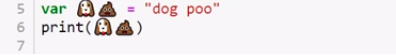
\includegraphics[width=0.6\linewidth,keepaspectratio]{s4tf4}
\end{center}

\item var $\pi$ = 3.1415925

\end{itemize}

\end{frame}

%%%%%%%%%%%%%%%%%%%%%%%%%%%%%%%%%%%%%%%%%%%%%%%%%%%%%%%%%%%
\begin{frame}[fragile] \frametitle{Variables}

\begin{itemize}
\item Values are never implicitly converted to another type.
\item Explicitly make an instance of the desired type.
\begin{lstlisting}
let label = "The width is "
let width = 94
let widthLabel = label + String(width)
\end{lstlisting}
\item To include values in strings: Write the value in parentheses, and write a backslash \lstinline|(\)| before the parentheses.
\begin{lstlisting}
let apples = 3
let oranges = 5
let appleSummary = "I have \(apples) apples."
let fruitSummary = "I have \(apples + oranges) pieces of fruit."
\end{lstlisting}
\item Use three double quotation marks \lstinline|(""")| for strings that take up multiple lines.
\end{itemize}


\end{frame}


%%%%%%%%%%%%%%%%%%%%%%%%%%%%%%%%%%%%%%%%%%%%%%%%%%%
\begin{frame}[fragile] \frametitle{Data Types}
\begin{itemize}
\item Supports all the common data types, like Integer, String, Float and Double. 
\item Assign any variable with a value, and its type will automatically be inferred by Swift.
\begin{lstlisting}
let marks = 63
let percentage = 70.0
var name = "Sushil"
\end{lstlisting}
\item Type can be specified explicitly as well.
\begin{lstlisting}
let weight: Double = 72.8
\end{lstlisting}
\item Swift will throw an error if the types do not match.
\end{itemize}
\end{frame}

%%%%%%%%%%%%%%%%%%%%%%%%%%%%%%%%%%%%%%%%%%%%%%%%%%%
\begin{frame}[fragile] \frametitle{Data Structures}
Supports both list and dictionary data structures just like Python, Dict syntax is different though.
\begin{lstlisting}
var shoppingList = ["catfish", "water", "tulips", "blue paint"]
shoppingList[1] = "bottle of water"
shoppingList.append("red apple")
print(shoppingList)

var occupationsDict = [
    "Malcolm": "Captain",
    "Kaylee": "Mechanic",
]
occupationsDict["Jayne"] = "Public Relations"
\end{lstlisting}


\end{frame}

%%%%%%%%%%%%%%%%%%%%%%%%%%%%%%%%%%%%%%%%%%%%%%%%%%%
\begin{frame}[fragile] \frametitle{Data Structures}
Empty creation

\begin{lstlisting}
let emptyArray = [String]()
let emptyDictionary = [String: Float]()
\end{lstlisting}

If type information can be inferred, you can write an empty array as [] and an empty dictionary as [:]
\begin{lstlisting}
shoppingList = []
occupations = [:]
\end{lstlisting}

\end{frame}


%%%%%%%%%%%%%%%%%%%%%%%%%%%%%%%%%%%%%%%%%%%%%%%%%%%
\begin{frame}[fragile] \frametitle{Working with Loops}

\begin{itemize}
\item Supports all the conventional looping mechanisms (for, while, etc.) but also implements some variations of its own.
\item The three dots in the first example are used to denote ``range'' in Swift. \lstinline|a...b| be values between a and b.
\item If we want to exclude the last number, we can just change the three dots to \lstinline|..<| like \lstinline|a..<b|
\item No indentation as Python but uses curly brackets ``{}'' like C.
\end{itemize}

\begin{lstlisting}
for i in 0...5{
	print(i)
}
var somelist = [1,44,5,6,342]
for item in somelist{
	print(item*2)
}
\end{lstlisting}
\end{frame}


%%%%%%%%%%%%%%%%%%%%%%%%%%%%%%%%%%%%%%%%%%%%%%%%%%%
\begin{frame}[fragile] \frametitle{Working with Loops}

Dictionaries are an unordered collection, so their keys and values are iterated over in an arbitrary order.

\begin{lstlisting}
let interestingNumbers = [
    "Prime": [2, 3, 5, 7, 11, 13],
    "Fibonacci": [1, 1, 2, 3, 5, 8],
    "Square": [1, 4, 9, 16, 25],
]
var largest = 0
for (kind, numbers) in interestingNumbers {
    for number in numbers {
        if number > largest {
            largest = number
        }
    }
}
print(largest) // Prints "25"
\end{lstlisting}
\end{frame}

%%%%%%%%%%%%%%%%%%%%%%%%%%%%%%%%%%%%%%%%%%%%%%%%%%%
\begin{frame}[fragile] \frametitle{Working with Loops}

\begin{itemize}
\item Use while to repeat a block of code until a condition changes. 
\item The condition of a loop can be at the end instead, ensuring that the loop is run at least once.
\end{itemize}

\begin{lstlisting}
var n = 2
while n < 100 {
    n *= 2
}
print(n) // Prints "128"

var m = 2
repeat {
    m *= 2
} while m < 100
print(m) // Prints "128"
\end{lstlisting}
\end{frame}

%%%%%%%%%%%%%%%%%%%%%%%%%%%%%%%%%%%%%%%%%%%%%%%%%%%
\begin{frame}[fragile] \frametitle{Conditionals}

\begin{itemize}
\item Supports conditional statements like \lstinline|if, if..else|
\item Supports even the \lstinline|switch| statement
\end{itemize}

\begin{lstlisting}
let individualScores = [75, 43, 103, 87, 12]
var teamScore = 0
for score in individualScores {
    if score > 50 {
        teamScore += 3
    } else {
        teamScore += 1
    }
}
print(teamScore)
// Prints "11"
\end{lstlisting}
\end{frame}

%%%%%%%%%%%%%%%%%%%%%%%%%%%%%%%%%%%%%%%%%%%%%%%%%%%
\begin{frame}[fragile] \frametitle{Optionals}

\begin{itemize}
\item An optional value either contains a value or contains nil to indicate that a value is missing. 
\item Write a question mark \lstinline|(?)| after the type of a value to mark the value as optional.
\item If the variable \lstinline|name| has value then you can say \lstinline|name.count| as \lstinline|.count| is available on \lstinline|String|.
\item If the variable \lstinline|name| has \lstinline|nil| in it, trying to read name.count is unsafe and Swift won’t allow it. 
\item Instead, we must look inside the optional and see what’s there – a process known as unwrapping.
\end{itemize}

\begin{lstlisting}
var name: String? = nil

if let unwrapped = name {
    print("\(unwrapped.count) letters")
} else {
    print("Missing name.")
}
\end{lstlisting}

\end{frame}

%%%%%%%%%%%%%%%%%%%%%%%%%%%%%%%%%%%%%%%%%%%%%%%%%%%
\begin{frame}[fragile] \frametitle{Optionals}

\begin{itemize}
\item If the optional value is nil, the conditional is false and the code in braces is skipped. 
\item Otherwise, the optional value is unwrapped and assigned to the constant after let, which makes the unwrapped value available inside the block of code.
\item If the optional value is missing, the default value is used instead.
\end{itemize}

\begin{lstlisting}
let nickname: String? = nil
let fullName: String = "John Appleseed"
let informalGreeting = "Hi \(nickname ?? fullName)"

var optionalString: String? = "Hello"
print(optionalString == nil) // Prints "false"

var optionalName: String? = "John Appleseed"
var greeting = "Hello!"
if let name = optionalName {
    greeting = "Hello, \(name)"
}
\end{lstlisting}

\end{frame}

%%%%%%%%%%%%%%%%%%%%%%%%%%%%%%%%%%%%%%%%%%%%%%%%%%%
\begin{frame}[fragile] \frametitle{Switch}

Support any kind of data and a wide variety of comparison operations—they aren’t limited to integers and tests for equality.
 
\begin{lstlisting}
let vegetable = "red pepper"
switch vegetable {
case "celery":
    print("Add some raisins and make ants on a log.")
case "cucumber", "watercress":
    print("That would make a good tea sandwich.")
case let x where x.hasSuffix("pepper"):
    print("Is it a spicy \(x)?")
default:
    print("Everything tastes good in soup.")
}
// Prints "Is it a spicy red pepper?"
\end{lstlisting}

Notice how let can be used in a pattern to assign the value that matched the pattern to a constant.

\end{frame}


%%%%%%%%%%%%%%%%%%%%%%%%%%%%%%%%%%%%%%%%%%%%%%%%%%%
\begin{frame}[fragile] \frametitle{Functions}

\begin{itemize}
\item Diff w Python: Swift uses the func keyword instead of def and we explicitly mention the data types of the arguments and the return type of the function.
\item Curly brackets “{}” to denote the code block that belongs to this function.
\end{itemize}


\begin{center}
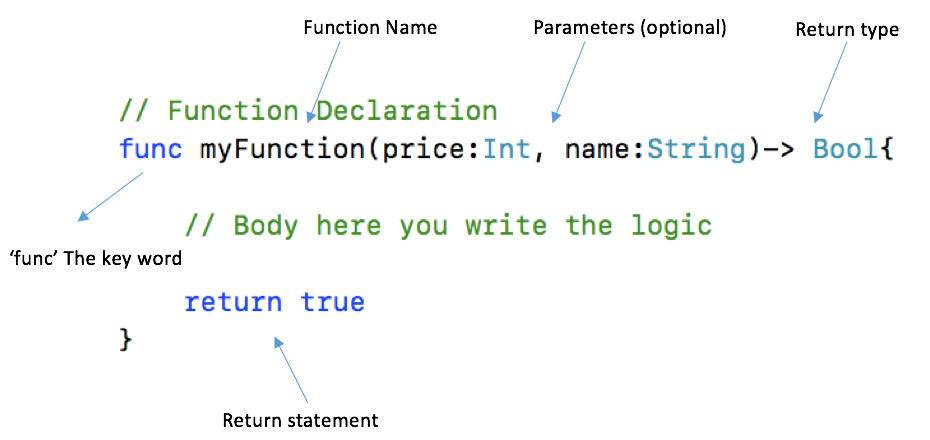
\includegraphics[width=0.8\linewidth,keepaspectratio]{s4tf5}
\end{center}

\end{frame}

%%%%%%%%%%%%%%%%%%%%%%%%%%%%%%%%%%%%%%%%%%%%%%%%%%%
\begin{frame}[fragile] \frametitle{Functions}

\begin{itemize}
\item By default, functions use their parameter names as labels for their arguments. 
\item Write a custom argument label before the parameter name, or write \_ to use no argument label.

\begin{lstlisting}
func greet(_ person: String, on day: String) -> String {
    return "Hello \(person), today is \(day)."
}
greet("John", on: "Wednesday")
\end{lstlisting}

\end{itemize}
\end{frame}

%%%%%%%%%%%%%%%%%%%%%%%%%%%%%%%%%%%%%%%%%%%%%%%%%%%
\begin{frame}[fragile] \frametitle{Functions}

\begin{lstlisting}
func calculateStatistics(scores: [Int]) -> (min: Int, max: Int, sum: Int) {
    var min = scores[0]
    var max = scores[0]
    var sum = 0
    for score in scores {
        if score > max {
            max = score
        } else if score < min {
            min = score
        }
        sum += score
    }
    return (min, max, sum) // tuple to make a compound value
}
let statistics = calculateStatistics(scores:[5,3,100,3 9])
print(statistics.sum) // Prints "120"
print(statistics.2) // Prints "120"
\end{lstlisting}
\end{frame}

%%%%%%%%%%%%%%%%%%%%%%%%%%%%%%%%%%%%%%%%%%%%%%%%%%%
\begin{frame}[fragile] \frametitle{Functions}
Functions can be nested. Nested functions have access to variables that were declared in the outer function.


\begin{lstlisting}
func returnFifteen() -> Int {
    var y = 10
    func add() {
        y += 5
    }
    add()
    return y
}
returnFifteen()
\end{lstlisting}


\end{frame}

%%%%%%%%%%%%%%%%%%%%%%%%%%%%%%%%%%%%%%%%%%%%%%%%%%%
\begin{frame}[fragile] \frametitle{Functions}

Functions are a first-class type. This means that a function can return another function as its value.
\begin{lstlisting}
func makeIncrementer() -> ((Int) -> Int) {
    func addOne(number: Int) -> Int {
        return 1 + number
    }
    return addOne
}
var increment = makeIncrementer()
increment(7)
\end{lstlisting}

\end{frame}


%%%%%%%%%%%%%%%%%%%%%%%%%%%%%%%%%%%%%%%%%%%%%%%%%%%
\begin{frame}[fragile] \frametitle{Functions}
A function can take another function as one of its arguments.

\begin{lstlisting}
func hasAnyMatches(list: [Int], condition: (Int) -> Bool) -> Bool {
    for item in list {
        if condition(item) {
            return true
        }
    }
    return false
}
func lessThanTen(number: Int) -> Bool {
    return number < 10
}
var numbers = [20, 19, 7, 12]
hasAnyMatches(list: numbers, condition: lessThanTen)
\end{lstlisting}

\end{frame}


%%%%%%%%%%%%%%%%%%%%%%%%%%%%%%%%%%%%%%%%%%%%%%%%%%%
\begin{frame}[fragile] \frametitle{Functions}
\begin{itemize}
\item Functions are actually a special case of closures: blocks of code that can be called later. 
\item The code in a closure has access to things like variables and functions that were available in the scope where the closure was created, even if the closure is in a different scope when it is executed.
\item You can write a closure without a name by surrounding code with braces ({}). Use in to separate the arguments and return type from the body.
\end{itemize}

\begin{lstlisting}
numbers.map({ (number: Int) -> Int in
    let result = 3 * number
    return result
})
\end{lstlisting}

\end{frame}


%%%%%%%%%%%%%%%%%%%%%%%%%%%%%%%%%%%%%%%%%%%%%%%%%%%
\begin{frame}[fragile] \frametitle{Functions}
\begin{itemize}
\item You have several options for writing closures more concisely. 
\item When a closure’s type is already known, such as the callback for a delegate, you can omit the type of its parameters, its return type, or both. 
\item Single statement closures implicitly return the value of their only statement.
\end{itemize}

\begin{lstlisting}
let mappedNumbers = numbers.map({ number in 3 * number })
print(mappedNumbers)
// Prints "[60, 57, 21, 36]"
\end{lstlisting}

\end{frame}

%%%%%%%%%%%%%%%%%%%%%%%%%%%%%%%%%%%%%%%%%%%%%%%%%%%
\begin{frame}[fragile] \frametitle{Functions}
\begin{itemize}
\item You can refer to parameters by number instead of by name—this approach is especially useful in very short closures. 
\item A closure passed as the last argument to a function can appear immediately after the parentheses. 
\item When a closure is the only argument to a function, you can omit the parentheses entirely.
\end{itemize}

\begin{lstlisting}
let sortedNumbers = numbers.sorted { $0 > $1 }
print(sortedNumbers)
// Prints "[20, 19, 12, 7]"
\end{lstlisting}

\end{frame}

%%%%%%%%%%%%%%%%%%%%%%%%%%%%%%%%%%%%%%%%%%%%%%%%%%%
\begin{frame}[fragile] \frametitle{Objects and Classes}
\begin{itemize}
\item Use class followed by the class’s name to create a class. 
\item A property declaration in a class is written the same way as a constant or variable declaration, except that it is in the context of a class. 
\item Likewise, method and function declarations are written the same way.
\end{itemize}

\begin{lstlisting}
class Shape {
    var numberOfSides = 0
    func simpleDescription() -> String {
        return "A shape with \(numberOfSides) sides."
    }
}
\end{lstlisting}

\end{frame}

%%%%%%%%%%%%%%%%%%%%%%%%%%%%%%%%%%%%%%%%%%%%%%%%%%%
\begin{frame}[fragile] \frametitle{Objects and Classes}
\begin{itemize}
\item Create an instance of a class by putting parentheses after the class name. 
\item Use dot syntax to access the properties and methods of the instance.
\end{itemize}

\begin{lstlisting}
var shape = Shape()
shape.numberOfSides = 7
var shapeDescription = shape.simpleDescription()
\end{lstlisting}


\end{frame}


%%%%%%%%%%%%%%%%%%%%%%%%%%%%%%%%%%%%%%%%%%%%%%%%%%%
\begin{frame}[fragile] \frametitle{Init}
Use init to create initializer.

\begin{lstlisting}
var shape = Shape()
class NamedShape {
    var numberOfSides: Int = 0
    var name: String
    init(name: String) {
        self.name = name
    }
    func simpleDescription() -> String {
        return "A shape with \(numberOfSides) sides."
    }
}
\end{lstlisting}

\lstinline|self| is used to distinguish the name property from the name argument to the initializer. 
\end{frame}


%%%%%%%%%%%%%%%%%%%%%%%%%%%%%%%%%%%%%%%%%%%%%%%%%%%
\begin{frame}[fragile] \frametitle{De-Init}
\begin{itemize}
\item Use \lstinline|deinit| to create a deinitializer if you need to perform some cleanup before the object is deallocated.
\item Subclasses include their superclass name after their class name, separated by a colon. 
\item There is no requirement for classes to subclass any standard root class, so you can include or omit a superclass as needed.
\end{itemize}


\end{frame}


%%%%%%%%%%%%%%%%%%%%%%%%%%%%%%%%%%%%%%%%%%%%%%%%%%%
\begin{frame}[fragile] \frametitle{Override}
\begin{itemize}
\item Methods on a subclass that override the superclass’s implementation are marked with override—overriding a method by accident, without override, is detected by the compiler as an error. 
\item The compiler also detects methods with override that don’t actually override any method in the superclass.
\end{itemize}


\end{frame}

%%%%%%%%%%%%%%%%%%%%%%%%%%%%%%%%%%%%%%%%%%%%%%%%%%%
\begin{frame}[fragile] \frametitle{Override}

\begin{lstlisting}
class Square: NamedShape {
    var sideLength: Double
    init(sideLength: Double, name: String) {
        self.sideLength = sideLength
        super.init(name: name)
        numberOfSides = 4
    }
    func area() -> Double {
        return sideLength * sideLength
    }
    override func simpleDescription() -> String {
        return "A square with sides of length \(sideLength)."
    }
}
let test = Square(sideLength: 5.2, name: "my test square")
test.area()
test.simpleDescription()
\end{lstlisting}

\end{frame}


%%%%%%%%%%%%%%%%%%%%%%%%%%%%%%%%%%%%%%%%%%%%%%%%%%%
\begin{frame}[fragile] \frametitle{Properties}

Properties can have a getter and a setter.

\begin{lstlisting}
class EquilateralTriangle: NamedShape {
    var sideLength: Double = 0.0
    var perimeter: Double {
        get {
            return 3.0 * sideLength
        }
        set {
            sideLength = newValue / 3.0
        }
    }
}
\end{lstlisting}


\end{frame}

%%%%%%%%%%%%%%%%%%%%%%%%%%%%%%%%%%%%%%%%%%%%%%%%%%%
\begin{frame}[fragile] \frametitle{Properties}

In the setter for perimeter, the new value has the implicit name newValue. You can provide an explicit name in parentheses after set.


\begin{lstlisting}
var triangle = EquilateralTriangle(sideLength: 3.1, name: "a triangle")
print(triangle.perimeter) // Prints "9.3"
triangle.perimeter = 9.9
print(triangle.sideLength) // Prints "3.3000000000000003"
\end{lstlisting}


\end{frame}

%%%%%%%%%%%%%%%%%%%%%%%%%%%%%%%%%%%%%%%%%%%%%%%%%%%
\begin{frame}[fragile] \frametitle{Properties}

The EquilateralTriangle init has following steps:
\begin{itemize}
\item Setting the value of properties that the subclass declares.
\item Calling the superclass’s initializer.
\item Changing the value of properties defined by the superclass. Any additional setup work that uses methods, getters, or setters can also be done at this point.
\end{itemize}

\begin{lstlisting}
class EquilateralTriangle: NamedShape {
    var sideLength: Double = 0.0

    init(sideLength: Double, name: String) {
        self.sideLength = sideLength
        super.init(name: name)
        numberOfSides = 3
    }
}
\end{lstlisting}

\end{frame}

%%%%%%%%%%%%%%%%%%%%%%%%%%%%%%%%%%%%%%%%%%%%%%%%%%%
\begin{frame}[fragile] \frametitle{Properties}

\begin{itemize}
\item Use \lstinline|willSet| and \lstinline|didSet| for code before and after property is being set.
\item The code is run any time the value changes outside of an initializer.
\end{itemize}

\begin{lstlisting}
class TriangleAndSquare {
    var triangle: EquilateralTriangle {
        willSet {
            square.sideLength = newValue.sideLength
        }
    }
    var square: Square {
        willSet {
            triangle.sideLength = newValue.sideLength
        }
    }
}
\end{lstlisting}
\end{frame}


%%%%%%%%%%%%%%%%%%%%%%%%%%%%%%%%%%%%%%%%%%%%%%%%%%%
\begin{frame}[fragile] \frametitle{Properties}

The class below ensures that the side length of its triangle is always the same as the side length of its square.

\begin{lstlisting}
class TriangleAndSquare {
    init(size: Double, name: String) {
        square = Square(sideLength: size, name: name)
        triangle = EquilateralTriangle(sideLength: size, name: name)
    }
}
var triangleAndSquare = TriangleAndSquare(size: 10, name: "another test shape")
print(triangleAndSquare.square.sideLength) // Prints "10.0"
print(triangleAndSquare.triangle.sideLength) // Prints "10.0"
triangleAndSquare.square = Square(sideLength: 50, name: "larger square")
print(triangleAndSquare.triangle.sideLength) // Prints "50.0"
\end{lstlisting}


\end{frame}

%%%%%%%%%%%%%%%%%%%%%%%%%%%%%%%%%%%%%%%%%%%%%%%%%%%
\begin{frame}[fragile] \frametitle{Optionals}

\begin{itemize}
\item Write \lstinline|?| before operations like methods, properties, and subscripting. 
\item If the value before the \lstinline|?| is \lstinline|nil|, everything after the \lstinline|?| is ignored and the value of the whole expression is \lstinline|nil|. 
\item Otherwise, the optional value is unwrapped, and everything after the \lstinline|?| acts on the unwrapped value. 
\item In both cases, the value of the whole expression is an optional value.
\end{itemize}

\begin{lstlisting}
let optionalSquare: Square? = Square(sideLength: 2.5, name: "optional square")
let sideLength = optionalSquare?.sideLength
\end{lstlisting}


\end{frame}

%%%%%%%%%%%%%%%%%%%%%%%%%%%%%%%%%%%%%%%%%%%%%%%%%%%
\begin{frame}[fragile] \frametitle{Enumeration}

\begin{itemize}
\item \lstinline|enum| is like a collection of constants where one of them is set at a time. 
\item Like classes and all other named types, enumerations can have methods associated with them.
\item By default, Swift assigns the raw values starting at zero and incrementing by one each time.
\item But you can change this behavior by explicitly specifying values. 
\end{itemize}

\end{frame}


%%%%%%%%%%%%%%%%%%%%%%%%%%%%%%%%%%%%%%%%%%%%%%%%%%%
\begin{frame}[fragile] \frametitle{Enumeration}
\begin{lstlisting}
enum Rank: Int {
    case ace = 1
    case jack
    func simpleDescription() -> String {
        switch self {
        case .ace:
            return "ace"
        case .jack:
            return "jack"
        default:
            return String(self.rawValue)
        }
    }
}
let ace = Rank.ace
let aceRawValue = ace.rawValue
\end{lstlisting}
In the example above, Ace is explicitly given a raw value of 1, and the rest of the raw values are assigned in order.

\end{frame}

%%%%%%%%%%%%%%%%%%%%%%%%%%%%%%%%%%%%%%%%%%%%%%%%%%%
\begin{frame}[fragile] \frametitle{Enumeration}

\begin{itemize}
\item Use the \lstinline|init?(rawValue:)| initializer to make an instance of an enumeration from a raw value. 
\item It returns either the enumeration case matching the raw value or nil if there is no matching Rank.
\end{itemize}

\begin{lstlisting}
if let convertedRank = Rank(rawValue: 3) {
    let threeDescription = convertedRank.simpleDescription()
}
\end{lstlisting}
\end{frame}

%%%%%%%%%%%%%%%%%%%%%%%%%%%%%%%%%%%%%%%%%%%%%%%%%%%
\begin{frame}[fragile] \frametitle{Structure}

\begin{itemize}
\item Use \lstinline|struct| to create a structure like in C++ (can have methods unlike in C)
\item the most important differences between structures and classes is that structures are always copied when they are passed around in your code, but classes are passed by reference.
\end{itemize}

\begin{lstlisting}
struct Card {
    var rank: Rank
    var suit: Suit
    func simpleDescription() -> String {
        return "The \(rank.simpleDescription()) of \(suit.simpleDescription())"
    }
}
let threeOfSpades = Card(rank: .three, suit: .spades)
let threeOfSpadesDescription = threeOfSpades.simpleDescription()
\end{lstlisting}
\end{frame}

%%%%%%%%%%%%%%%%%%%%%%%%%%%%%%%%%%%%%%%%%%%%%%%%%%%
\begin{frame}[fragile] \frametitle{Protocols}

Use \lstinline|protocol| to declare a protocol like Interface in Java.


\begin{lstlisting}
protocol ExampleProtocol {
    var simpleDescription: String { get }
    mutating func adjust()
}
\end{lstlisting}
\end{frame}

%%%%%%%%%%%%%%%%%%%%%%%%%%%%%%%%%%%%%%%%%%%%%%%%%%%
\begin{frame}[fragile] \frametitle{Protocols}

Classes, enumerations, and structs can all adopt protocols.

\begin{lstlisting}
class SimpleClass: ExampleProtocol {
    var simpleDescription: String = "A very simple class."
    var anotherProperty: Int = 69105
    func adjust() {
        simpleDescription += "  Now 100% adjusted."
    }
}
var a = SimpleClass()
a.adjust()
let aDescription = a.simpleDescription
\end{lstlisting}
\end{frame}

%%%%%%%%%%%%%%%%%%%%%%%%%%%%%%%%%%%%%%%%%%%%%%%%%%%
\begin{frame}[fragile] \frametitle{Protocols}

\begin{lstlisting}
struct SimpleStructure: ExampleProtocol {
    var simpleDescription: String = "A simple structure"
    mutating func adjust() {
        simpleDescription += " (adjusted)"
    }
}
var b = SimpleStructure()
b.adjust()
let bDescription = b.simpleDescription
\end{lstlisting}

\begin{itemize}
\item The \lstinline|mutating| keyword is to mark a method that modifies the structure. 
\item SimpleClass doesn’t need it because methods on a class can always modify the class.
\end{itemize}

\end{frame}


%%%%%%%%%%%%%%%%%%%%%%%%%%%%%%%%%%%%%%%%%%%%%%%%%%%
\begin{frame}[fragile] \frametitle{Extension}

\begin{itemize}
\item Use \lstinline|extension| to add functionality to an existing type, such as new methods and computed properties. 
\item You can use an extension to add protocol conformance to a type that is declared elsewhere, or even to a type that you imported from a library or framework.
\end{itemize}

\begin{lstlisting}
extension Int: ExampleProtocol {
    var simpleDescription: String {
        return "The number \(self)"
    }
    mutating func adjust() {
        self += 42
    }
}
print(7.simpleDescription)
// Prints "The number 7"
\end{lstlisting}
\end{frame}

%%%%%%%%%%%%%%%%%%%%%%%%%%%%%%%%%%%%%%%%%%%%%%%%%%%
\begin{frame}[fragile] \frametitle{Protocol}

\begin{itemize}
\item You can use a protocol name just like any other named type—for example, to create a collection of objects that have different types but that all conform to a single protocol.
\item Note that in such cases methods outside the protocol definition are not available.
\end{itemize}

\begin{lstlisting}
let protocolValue: ExampleProtocol = a
print(protocolValue.simpleDescription)
// Prints "A very simple class.  Now 100% adjusted."
// print(protocolValue.anotherProperty)  // Uncomment to see the error
\end{lstlisting}
\end{frame}

%%%%%%%%%%%%%%%%%%%%%%%%%%%%%%%%%%%%%%%%%%%%%%%%%%%
\begin{frame}[fragile] \frametitle{Protocol}

\begin{itemize}
\item Even though the variable \lstinline|protocolValue| has a runtime type of \lstinline|SimpleClass|, the compiler treats it as the given type of \lstinline|ExampleProtocol|. 
\item This means that you can’t accidentally access methods or properties that the class implements in addition to its protocol conformance.
\end{itemize}

\begin{lstlisting}
let protocolValue: ExampleProtocol = a
print(protocolValue.simpleDescription)
// Prints "A very simple class.  Now 100% adjusted."
// print(protocolValue.anotherProperty)  // Uncomment to see the error
\end{lstlisting}
\end{frame}

%%%%%%%%%%%%%%%%%%%%%%%%%%%%%%%%%%%%%%%%%%%%%%%%%%%
\begin{frame}[fragile] \frametitle{Error Handling}


Use throw to throw an error and throws to mark a function that can throw an error. 

\begin{lstlisting}
func send(job: Int, toPrinter printerName: String) throws -> String {
    if printerName == "Never Has Toner" {
        throw PrinterError.noToner
    }
    return "Job sent"
}
\end{lstlisting}


\end{frame}

%%%%%%%%%%%%%%%%%%%%%%%%%%%%%%%%%%%%%%%%%%%%%%%%%%%
\begin{frame}[fragile] \frametitle{Error Handling}

Use throw to throw an error and throws to mark a function that can throw an error. 

\begin{lstlisting}
func send(job: Int, toPrinter printerName: String) throws -> String {
    if printerName == "Never Has Toner" {
        throw PrinterError.noToner
    }
    return "Job sent"
}
\end{lstlisting}


\end{frame}


%%%%%%%%%%%%%%%%%%%%%%%%%%%%%%%%%%%%%%%%%%%%%%%%%%%
\begin{frame}[fragile] \frametitle{Error Handling}

\begin{itemize}
\item Use \lstinline|do-catch| to handle the error.
\item Inside the \lstinline|do| block, you mark code that can throw an error by writing \lstinline|try| in front of it.
\item Inside the \lstinline|catch| block, the error is automatically given the name \lstinline|error| unless you give it a different name. 
\end{itemize}

\begin{lstlisting}
do {
    let printerResponse = try send(job: 1040, toPrinter: "Bi Sheng")
    print(printerResponse)
} catch {
    print(error)
}
// Prints "Job sent"
\end{lstlisting}


\end{frame}

%%%%%%%%%%%%%%%%%%%%%%%%%%%%%%%%%%%%%%%%%%%%%%%%%%%
\begin{frame}[fragile] \frametitle{Error Handling}

\begin{itemize}
\item Provide multiple catch blocks that handle specific errors. 
\item Write a pattern after catch just as you do after case in a switch.
\end{itemize}

\begin{lstlisting}
do {
    let printerResponse = try send(job: 1440, toPrinter: "Gutenberg")
    print(printerResponse)
} catch PrinterError.onFire {
    print("I'll just put this over here, with the rest of the fire.")
} catch let printerError as PrinterError {
    print("Printer error: \(printerError).")
} catch {
    print(error)
}
// Prints "Job sent"
\end{lstlisting}


\end{frame}

%%%%%%%%%%%%%%%%%%%%%%%%%%%%%%%%%%%%%%%%%%%%%%%%%%%
\begin{frame}[fragile] \frametitle{Error Handling}

\begin{itemize}
\item Another way to handle errors is to use \lstinline|try?| to convert the result to an optional. 
\item If the function throws an error, the specific error is discarded and the result is \lstinline|nil|. 
\item Otherwise, the result is an optional containing the value that the function returned.
\end{itemize}

\begin{lstlisting}
let printerSuccess = try? send(job: 1884, toPrinter: "Mergenthaler")
let printerFailure = try? send(job: 1885, toPrinter: "Never Has Toner")
\end{lstlisting}
\end{frame}

%%%%%%%%%%%%%%%%%%%%%%%%%%%%%%%%%%%%%%%%%%%%%%%%%%%
\begin{frame}[fragile] \frametitle{Error Handling}

\begin{itemize}
\item Use \lstinline|defer| to write a block of code that is executed after all other code in the function, just before the function returns. 
\item The code is executed regardless of whether the function throws an error. 
\item You can use \lstinline|defer| to write setup and cleanup code next to each other, even though they need to be executed at different times.
\end{itemize}

\end{frame}

%%%%%%%%%%%%%%%%%%%%%%%%%%%%%%%%%%%%%%%%%%%%%%%%%%%
\begin{frame}[fragile] \frametitle{Error Handling}

\begin{lstlisting}
var fridgeIsOpen = false
let fridgeContent = ["milk", "eggs", "leftovers"]

func fridgeContains(_ food: String) -> Bool {
    fridgeIsOpen = true
    defer {
        fridgeIsOpen = false
    }

    let result = fridgeContent.contains(food)
    return result
}
fridgeContains("banana")
print(fridgeIsOpen)
// Prints "false"
\end{lstlisting}
\end{frame}

%%%%%%%%%%%%%%%%%%%%%%%%%%%%%%%%%%%%%%%%%%%%%%%%%%%
\begin{frame}[fragile] \frametitle{Generics}

\begin{itemize}
\item To define meta-type, like Templates in C++
\item Write a name inside angle brackets to make a generic function or type.
\end{itemize}

\begin{lstlisting}
func makeArray<Item>(repeating item: Item, numberOfTimes: Int) -> [Item] {
    var result = [Item]()
    for _ in 0..<numberOfTimes {
        result.append(item)
    }
    return result
}
makeArray(repeating: "knock", numberOfTimes: 4)
\end{lstlisting}
\end{frame}

%%%%%%%%%%%%%%%%%%%%%%%%%%%%%%%%%%%%%%%%%%%%%%%%%%%
\begin{frame}[fragile] \frametitle{Generics}

You can make generic forms of functions and methods, as well as classes, enumerations, and structures.

\begin{lstlisting}
// Reimplement the Swift standard library's optional type
enum OptionalValue<Wrapped> {
    case none
    case some(Wrapped)
}
var possibleInteger: OptionalValue<Int> = .none
possibleInteger = .some(100)
\end{lstlisting}
\end{frame}

%%%%%%%%%%%%%%%%%%%%%%%%%%%%%%%%%%%%%%%%%%%%%%%%%%%
\begin{frame}[fragile] \frametitle{Generics}

Use \lstinline|where| to specify requirements, eg, the type to implement a protocol, two types to be the same, etc.

\begin{lstlisting}
func anyCommonElements<T: Sequence, U: Sequence>(_ lhs: T, _ rhs: U) -> Bool
    where T.Element: Equatable, T.Element == U.Element
{
    for lhsItem in lhs {
        for rhsItem in rhs {
            if lhsItem == rhsItem {
                return true
            }
        }
    }
    return false
}
anyCommonElements([1, 2, 3], [3])
\end{lstlisting}
% Writing \lstinline|<T: Equatable>| is the same as writing \lstinline|<T> ... where T: Equatable|.
\end{frame}


%%%%%%%%%%%%%%%%%%%%%%%%%%%%%%%%%%%%%%%%%%%%%%%%%%%
\begin{frame}[fragile] \frametitle{Python in Swift}

\begin{itemize}
\item Import useful Python libraries from Swift, call their functions, and convert values between Swift and Python seamlessly.
\item In Swift for Tensorflow its \lstinline|import PythonKit|
\end{itemize}

\begin{lstlisting}
import Python

// Load numpy from Python
let np = Python.import("numpy")

// Create an array of zeros
var zeros = np.ones([2, 3])
print(zeros)
\end{lstlisting}
\end{frame}
